\documentclass[a4paper, 12pt]{report}
%================================================================
\usepackage{color,amsmath,amsfonts,amssymb,epsfig,hyperref}
\usepackage{graphicx}
\usepackage{dsfont}
\usepackage[latin1]{inputenc}
\usepackage[T1]{fontenc}
\usepackage[english]{babel}
\usepackage{pdfpages}
%====================================
% \textheight 22cm
%% \doublespace
%  \oddsidemargin 0 cm
%  \evensidemargin +1.5cm
%  \textwidth 16cm
% \topmargin 0 cm
%============================================
% Figures
%============================================
\newcommand{\figsstit}[2]{
\begin{figure}[hbtp]
\centerline{
    \hbox{ \includegraphics[scale=#2]{#1} }
}
\end{figure}}
%============================================
\newcommand{\figscale}[4]{
\begin{figure}[hbtp]
\centerline{
    \hbox{ \includegraphics[scale=#4]{#1} }
}
\begin{center}
\parbox{14 cm}
{
    \caption{\protect\small\it  {#2}}
    \label {#3}
}
\end{center}

\end{figure}}

%==================================================
\newcommand\algo[1]%
{
    \begin{center} %
    \begin{tabular} {||p{10 cm}l ||}%
    \hline
               #1 &  \\
    \hline
    \end{tabular}
    \vspace{12pt}
    \end{center}
}


%==============================================
\newcommand{\prob}[1]{\mathds{P}\left( #1 \right)}
\newcommand{\esp}[1]{\mathds{E}\left[ #1 \right]}
\newcommand{\var}[1]{\mathrm{var}\left( #1 \right)}
\newcommand{\cov}[1]{\mathrm{cov}\left( #1 \right)}
\newcommand{\diag}[1]{\mathrm{diag}\left( #1 \right)}
\newcommand{\trace}[1]{\mathrm{trace}\left( #1 \right)}
\newcommand{\card}[1]{\left| #1 \right|}
\newcommand{\myemph}[1]{\emph{\color{red}#1}}

%%============================================================================
\def\thesection{\arabic{section}}
%\def\thesubsection{\arabic{section}.\arabic{subsection}}
%\def\thesubsubsection{\arabic{section}.\arabic{subsection}.\arabic{subsubsection}}
%\def\thefigure{\arabic{figure}}
%\def\theequation{\arabic{equation}}
%\def\theexercice{\arabic{exercice}}
%\def\theexample{\arabic{example}}
%\def\theproof{\arabic{proof}}

%===============================================
\newtheorem{property}{Properties}
\newtheorem{remark}{Remark}
\newtheorem{theorem}{Theorem}
\newtheorem{definition}{Definition}
\newtheorem{example}{Example}
\newtheorem{lemme}{Lemme - \thelemme}
\newtheorem{proof}{Proof - \theproof}
\newenvironment{TAB}{\begin{table}[[hbt] \center \leavevmode}{\end{table}}
%%============================================================================
%\renewcommand\arraystretch{1.6}

\def\ua{\underline a}
\def\ub{\underline b}
\def\uB{\underline B}
\def\uH{\underline H}
\def\ur{\underline r}
\def\us{\underline s}
\def\ux{\underline x}
\def\uX{\underline X}
\def\uZ{\underline Z}
\def\utheta{\underline \theta}



\def\tn{\mathrm{TN}}
\def\fn{\mathrm{FN}}
\def\tp{\mathrm{TP}}
\def\fp{\mathrm{FP}}
\def\tpn{\mathrm{tPN}}
\def\tnn{\mathrm{tNN}}
\def\tdn{\mathrm{tDN}}

\def\precision{\mathrm{\color{red}Precision}}
\def\recall{\mathrm{\color{red}Recall}}
\def\fscore{{\color{red}F\mathrm{-score}}}
\def\far{\mathrm{FAR}}
\def\mdr{\mathrm{MDR}}
\def\vdr{\mathrm{VDR}}
\def\ci{\mathrm{CI}}
\def\pfa{P_{\mathrm{FA}}}
\def\pd{P_{\mathrm{D}}}
\def\loc{\mathrm{LOC}}

\def\SNR{\mathrm{SNR}}
\def\crb{\mathrm{CRB}}
\def\fim{\mathrm{FIM}}

\def\auc{\mathrm{AUC}}
\def\aec{\mathrm{aec}}



\def\void{{\small void}}
\def\nomeaning{{\small meaningless}}
\def\unknown{{\small unknown}}
\def\MSC{\mathrm{MSC}}
\def\hMSC{\widehat{\MSC}}%{\MSC}} 
\def\ellk{{k}}
\def\SOI{common signal part }
\def\absGamma{\Phi}

%============== colors ========================
\definecolor{enstrouge}{RGB}{212,65,84}
\definecolor{lightorange}{RGB}{235,226,52}
\definecolor{greennoise}{RGB}{243,42,255}
\definecolor{lightred}{RGB}{255,181,183}
\definecolor{light-grey}{rgb}{0.95,0.95,0.95}
\definecolor{peach}{rgb}{0.98,0.49,0.25}
\definecolor{burntorange}{rgb}{0.79,0.37,0}
\definecolor{light-yellow}{rgb}{1,1,0.92}

\definecolor{light-green}{RGB}{231,255,145}
\definecolor{enstorange}{RGB}{255,214,10}
\definecolor{enstrouge}{RGB}{212,65,84}
\definecolor{grey}{RGB}{204,204,204}
\definecolor{blue}{RGB}{0,0,255}
\definecolor{almost-black}{RGB}{100,100,100}
\definecolor{violet}{rgb}{0.4,0,0.4}
\definecolor{cyan}{RGB}{0,255,255}
\definecolor{magenta}{RGB}{243,42,255}

\def\degree{^{\circ}}
\def\simiid{\stackrel{\mathrm{i.i.d.}}{\sim}}
\def\simind{\stackrel{\mathrm{ind.}}{\sim}}

 
%%%============================================================================
%%\def\thesection{\arabic{section}}
%%\def\thefigure{\arabic{figure}}
%%\def\theequation{\arabic{equation}}
%%\def\theexercice{\arabic{exercice}}
%%\def\theequation{\arabic{exercice}.\arabic{equation}}
%%%============================================================================
%%\newcounter{auxiliaire}
%%%%%%%%% comment
%%\setcounter{auxiliaire}{\theenumi}
%%\end{enumerate}
%% TEXTE
%%\begin{enumerate}
%%\setcounter{enumi}{\theauxiliaire}
%%%============================================================================

 \bibliographystyle{plain} 

\begin{document}
 \sloppy
 \tableofcontents
%=======================================================
%=======================================================



%=======================================================
%=======================================================
\chapter{Main part}

In this study we are interested by the station design in term of parameter accuracy, and more particularly on the accuracy of the azimuth. In short, in presence of only pure coherent acoustic waves, it is clear that the best design is to locate sensors at far as possible. For which reason could we take into account an upper bound on the aperture ? 

Regarding the size of the station and the distance of the source, a possible phenomena, which could induce a limitation on the station aperture in presence of a coherent acoustic signal, is that the loss of coherence (LOC) which usually increases when the distance between sensors increases.

For conducting this study the 3 points following program has been considered:
\begin{itemize}
 \item
choosing an index to evaluate the accuracy of the station. A commonly used index is the Cramer-Rao bound (CRB). Typically that depends on the geometry of the station, the level of noise and the LOC features. A summary of the CRB could be the area/volume of the confidence ellipsoid.

 \item
choosing features to characterize a geometry. We have retained (i) the isotropy and (ii) the uniform distribution of the inter-distances. The isotropy is easy to check and also it is simple to correct if necessary by adding 2 sensors (resp. 3) for 2D station (resp. 3D station).

We can not answer to the good effect or not of the inter-distance uniformity because that depends on the LOC model. Therefore we have to validate a such model.

\item
validating a LOC model.

The used LOC feature is the magnitude square coherence (MSC). This index has the interesting property to be between 0 and 1, and equal to 1 iff the two signals are spatially coherent.

	The approach to determine the LOC model is based on the observation analysis. It is conducted as it follows: we consider the station I37 which consists of 10 sensors with 45 uniformly disibuted inter-distances. We base the analysis on the presence of a quasi-permanent coherent acoustical signal, saying the microbarom, in a frequency bandwidth large enough between 0.05 to 3 Hz. 

For a given frequency, we select the portions of signals where the MSC is greater than 0.8 on the three nearest sensors and study the decay of the MSC along the inter-distance values.

\end{itemize}



\begin{remark}[on the noise]
Typical station aperture  is 2 km. Noise is mainly due to the wind.
\begin{itemize}
\item
Therefore we assume that the noises are spatially uncorrelated regarding the sensor inter-distances.
\item
On the other hand, we assume that the noise levels are identical on all sensors. Although that is not realistic, it is worth to notice that the noise level is not directly related to the inter-distances between sensors. It follows that, for the station design understanding, we can consider there is no loss of generalities to assume that.
\end{itemize}
\end{remark}

\begin{remark}[on the coherent source]
To be able to study the LOC, we need a permanent source. The microbarom could play this role in many stations, but also gas-flare could be used in IS31.
\end{remark}

\begin{remark}[on the isotropy]
If $X$ denotes $d\times M$ matrix whose the $m$-th column if the coordinates of the $m$-th sensor (in any  system of coordinates), the delays are given by the linear model w.r.t. the slowness vector $\theta$ that writes:
\begin{eqnarray*}
 \tau &=& X\theta+\mathrm{noise}
\end{eqnarray*}
It is shown that in the absence of LOC, the station is isotrope w.r.t. the components of the slowness vector iff 
\begin{eqnarray}
 \label{eq:isotropy-condition}
XX^{T}&\propto&I_{d}
\end{eqnarray}

It follows that  given an arbitrary array with $M$ sensors in $\mathds{R}^{d}$ it is always possible to move any $d$ locations in such a way the new array is isotrope, i.e. verifies \eqref{eq:isotropy-condition}, see annex.

It is worth to notice that this isotropy is related to the 3 components of the slowness vector. If we used another parametrization, as for example azimuth, elevation, velocity we have to reconsidered the solution taking into account the Jacobian of the transformation.

\end{remark}

\begin{remark}[on the geometry]
In the absence of LOC, we will see below that the best performances are associated with inter-distances as large as possible. In this case the maximization of the minimal distance leads to locate the sensors on a circle. But in this case the distribution of the distances is not uniform. It follows that in presence of LOC, several sensors are concern with the same LOC. It seems (it is not a proof) that a rule could be to locate the sensors in such a way that the distances are more uniform (see figure \ref{fig:uniforinterdistances}).

\figscale{../figures/uniforinterdistances.pdf}{Sensor locations with inter distances}{fig:uniforinterdistances}{0.9}

\end{remark}


\newpage\clearpage
%=======================================================
 \section{LOC model}
%=======================================================
%=======================================================
\subsection{Case of 2 sensors}
By definition, two signals arriving on a two different locations are said non-coherent signals, or called noises, if they are spatially uncorrelated. More specifically if $x_{1}(t)$ and $x_{2}(t)$ denote the respective stationary signals observed in to different locations, the coherence level is defined by the magnitude square coherence:
\begin{eqnarray*}
 \MSC(f)&=&\frac{|S_{12}(f)|^{2}}{S_{11}(f)S_{22}(f)}
\end{eqnarray*}
where $S_{11}(f)$ and $S_{22}(f)$ denote the spectral densities of $x_{1}(t)$ and $x_{2}(t)$, and $S_{12}(f)$ the cross-spectrum. 
The MSC is only defined when the denominator is different of 0.

It is well known that $\MSC(f)\leq 1$. 
\begin{definition}[coherence - I]
\label{def:coherence2sensors}
When $\MSC(f)=1$, we say that the 2 signals are perfectly coherent, if not we speak of loss of coherence (LOC). 
\end{definition}


It is shown that the  $\MSC(f)$ between the two signals is 1, if and only if it exists a filter, with impulse response $g(t)$, such that $x_{1}(t)=g_{1}(t)\star x_{2}(t)$. A particular case is $g(t)=\delta(t-t_{0})$ which corresponds to the pure delay $t_{0}$.


  \medskip
 When $\MSC(f)=0$ we say that the 2 signals are spatially uncorrelated or non coherent. In the following we usually consider that noises are non coherent.



%=======================================================
\subsection{Case of $M$ sensors}
We consider a station with $M$ sensors. There is only one acoustic source faraway from the station, in such a way it can be considered as planar wave. This source is called in the following signal of interest (SOI). Therefore the $M$-ary signal  writes: 
\begin{eqnarray*}
x(t)  =  \underbrace{s(t;\theta)}_{\text{SOI: acoustic signal}} &+& \underbrace{w(t)}_{\text{noise}}
\end{eqnarray*}
where $\theta$ denotes the 3D slowness vector. Under  pure delay assumption we can write for the $m$-th sensor located in $r_{m}$:
\begin{eqnarray}
\label{eq:mthentryofst}
s_{m}(t;\theta)&=&s(t-r_{m}^{T}\theta)
\end{eqnarray}

It follows  that, under the assumption  that $s(t)$ is stationary random process with spectral density $\gamma_{s}(f)$, the spectral matrix of the $M$-ary process $s(t)$, whose the $m$-th entry is \eqref{eq:mthentryofst}, writes:
\begin{eqnarray*}
\Gamma_{s}(f)&=&\gamma_{s}(f)d(f)d^{H}(f)
\end{eqnarray*}
where $d(f)$ is a $M$-ary vector whose the $m$-entry writes $e^{-2j\pi fr_{m}^{T}\theta}$. Clearly the matrix $\Gamma_{s}(f)$ is of rank 1.  That represents the general definition of the coherence. 
\begin{definition}[coherence - II]
\label{def:coherenceMsensors}
$M$ stationary signals are said coherent if their spectral matrix is of rank 1 . 
\end{definition}

This definition is in accordance with the definition \ref{def:coherence2sensors} given for 2 sensors. 

\begin{theorem}[fundamental property]
For any frequency $f$, the spectral matrix is positive.
\end{theorem}


We assume that the $M$-ary noise $w(t)$ is temporally and spatial white. That writes $\esp{w(t)w^{T}(t')}=\sigma^{2}\delta(t-t')$, therefore its spectral matrix writes $\sigma^{2}I_M$ for any frequency. Assuming that the noise and the SOI are not correlated, it follows that the spectral matrix of the observation writes $\Gamma_{x}(f)= \gamma_{s}(f)d(f)d^{H}(f) + \sigma^{2}I_M$ that can be rewritten:
\begin{eqnarray}
\label{eq:generaldensitymatrixwithLOC}
 \Gamma_{x}(f)&=& \gamma_{s}(f)D(f)C(f)D^{H}(f) + \sigma^{2}I_M
\end{eqnarray}
where $D(f)$ is an $M$-ary diagonal matrix whose the $m$-th diagonal entry writes $D_{m,m}=e^{-2j\pi f r_{m}^{T}\theta }$ and where $C(f)=\mathds{1}\mathds{1}^{T}$. The LOC is then characterized by a matrix $C(f)$ which is no more of rank 1,  but must be positive and with diagonal element equal to $1$. 

\medskip
It follows that, for a pure delay and in the absence of LOC, taken $C(f)=\mathds{1}\mathds{1}^{T}$ in expressed in \eqref{eq:generaldensitymatrixwithLOC}, the MSC between any  sensor pair $(m,m')$ writes:
\begin{eqnarray*}
 \MSC_{m,m'}(f)&=& \frac{\gamma_{s}^{2}(f)}{(\gamma_{s}(f)+\sigma^{2})(\gamma_{s}(f)+\sigma^{2})}
\end{eqnarray*}
Therefore, in presence of noise, the MSC level is no more equal to $1$. In more general case:
\begin{eqnarray*}
 \MSC_{m,m'}(f)&=& \frac{\gamma_{s}^{2}(f)\, C_{m,m'}(f)}{(\gamma_{s}(f)+\sigma^{2})(\gamma_{s}(f)+\sigma^{2})}
\end{eqnarray*}



\begin{remark}
Coherence is not only restricted to the case of pure delays. Perfect coherence is also verified for filtering signals.
\end{remark}


\begin{remark}
Noise induces a LOC.
\end{remark}

%=======================================================
\subsection{Discrete domain}

All signals are real and sampled at the sampling frequency  $F_{s}=20$ Hz. After sampling we obtain $x_{n}=x(n/F_{s})$. For $k=0$ to $(N-1)$ we consider the $M$-ary discrete Fourier transform:
 \begin{eqnarray*}
 X_{k}&=&\frac{1}{\sqrt{N}}\sum_{n=0}^{N-1}x_{n}\,e^{-2j\pi n f_{k}}
    \quad\mathrm{where}\quad
 f_{k}=kF_{s}/N
 \end{eqnarray*}
We let $K=N/2$.
For $K$ great enough, $X_{1}$, $\ldots$, $X_{K}$ is a sequence of  $M$-ary independent circularly gaussian random vectors with zero-mean and respective covariance:
\begin{eqnarray}
\label{eq:spectralmatrixpuredelay}
\Gamma_{k}(\alpha)&=&\gamma_{k}d_{k}(\theta)d_{k}^{H}(\theta)+\sigma^{2}I_{M}
%\diag{\begin{matrix}\sigma_{1},\ldots,\sigma_{M}\end{matrix}}
\end{eqnarray}
where $d_{k}(\theta)$ is an $M$-ary vector whose the $m$-th entry writes $D_{k,m}=e^{-2j\pi f_{k} r_{m}^{T}\theta }$ and where $\gamma_{k}=\gamma_{s}(f_{k})$.

The expression \eqref{eq:spectralmatrixpuredelay} can be rewritten:
\begin{eqnarray}
\label{eq:spectralmatrixLOC}
\Gamma_{k}(\alpha)&=&\gamma_{k}D_{k}(\theta)\, C_{k}\,D_{k}^{H}(\theta)+\sigma^{2}I_{M}
%\diag{\begin{matrix}\sigma_{1},\ldots,\sigma_{M}\end{matrix}}
\end{eqnarray}
where $D_{k}(\theta)$ is an $M$-ary diagonal matrix whose the $m$-th diagonal entry writes $D_{k,m,m'}=e^{-2j\pi f_{k} r_{m}^{T}\theta }$ and where $C_{k}=\mathds{1}\mathds{1}^{T}$ which is a rank 1 matrix. Under LOC, $C_{k}$ is no more a rank 1 projector,  but must be positive and such that $C_{k,m,m}=1$.

From \eqref{eq:spectralmatrixLOC}, we get:
\begin{eqnarray*}
 \Gamma_{k,m,m'}&=& \gamma_{k}C_{k,m,m'}e^{-2j\pi f_{k} (r_{m}-r_{m'})^{T}\theta }+\sigma^{2}\delta_{m,m'}
\end{eqnarray*}


We let $\SNR_{k}=\gamma_{k}/\sigma^2$ the signal-to-noise ratio at the frequency $f_{k}$. It follows that the MSC at the frequency $f_{k}$  between any two sensors writes:
\begin{eqnarray}
\label{eq:MSCgeneralmodel}
 \MSC_{k,m,m'}&=& \frac{1}{(1+\SNR_{k}^{-1})^2}\,|C_{k,m,m'}|^{2}
\end{eqnarray}
It follows that the MSC could be less than 1 on one hand to the presence of noise and on the other to the LOC of the acoustic wave.


A commonly used model for the LOC of the acoustic source is for $1\leq m\leq M$ and $1\leq m'\leq M$:
\begin{eqnarray}
 \label{eq:CkwithGauss}
 C_{k,m,m'} &=&e^{-2\pi^2f_k^2(r_{m}-r_{m'})^TS_{\theta}(r_{m}-r_{m'})}
\end{eqnarray}
where $S_{\theta}$ is a $3\times 3$ covariance matrix depending on 3 free parameters. Using \eqref{eq:MSCgeneralmodel}, we get:
\begin{eqnarray}
\label{eq:MSCgaussianmodelwithnoise}
 \log \MSC_{k,m,m'}&=& -2 \log(1+\SNR_{k}^{-1})
-4\pi^2f_k^2(r_{m}-r_{m'})^TS_{\theta}(r_{m}-r_{m'})
\end{eqnarray}
In the simple case where $S_{\theta}$ is proportional to the identity, this expression simplifies as:
\begin{eqnarray}
\label{eq:logMSCgaussianmodel}
 \log \MSC_{k,m,m'}&=& \beta_{0}+\beta_{1} f_k^2 d_{m,m'}^2
%-4\pi^2f_k^2(r_{m}-r_{m'})^TS_{\theta}(r_{m}-r_{m'})
\end{eqnarray}
where we have assumed that the SNR does not depend on $k$ and writes:
\begin{eqnarray*}
 \SNR&=&\frac{1}{e^{- \beta_{0}/2}-1}
\end{eqnarray*}


\subsubsection{Likelihood function}
In summary   we can write that:
\begin{eqnarray*}
 (X_{1},\ldots,X_{K}) &\sim&\prod_{k=1}^{K}\mathcal{N}_{c}(x_{k};0_{M},\Gamma_{k}(\alpha))
\end{eqnarray*}
and the likelihood writes:
\begin{eqnarray}
 \label{eq:likelihood-function}
 \mathcal{L}(\alpha)&=&
 \sum_{k=1}^{K}\log\det\Gamma_{k}(\alpha)+\trace{\Gamma_{k}^{-1}(\alpha)X_{k}X_{k}^{T}}
\end{eqnarray}
where the parameter $\alpha$ consists of
\begin{eqnarray}
\alpha&=&
\{
\theta_{1},\theta_{2},\theta_{3},\gamma_{1},\ldots,\gamma_{K},S_{\theta},\sigma^{2}
\}
\in \mathds{R}^{3}\times\mathds{R}^{+K}\times   \mathcal{M}_{3}^{+}\times \mathds{R}^{+}
\end{eqnarray}
where $\mathcal{M}_{3}^{+}$ is the set of $3\times 3$ positive matrices. The size of the parameter $\alpha$ is $K+7$ whereas the number of observations is $2MK$.


Another way is to characterize the slowness by azimuth, elevation and velocity and the LOC by the respective standard deviations of them, see expression \eqref{eq:theta2aec}.
%=======================================================
 \section{LOC study: numerical results}
%=======================================================
%=======================================================
The objective of this section is to validate, by numerical results, the simple relationship between the LOC and the distance given by the expression \eqref{eq:logMSCgaussianmodel}, that we rewrite below:
\begin{eqnarray}
\label{eq:simplemodelMSC}
 \log \MSC_{k,m,m'}&=& \beta_{0}+\beta_{1} f_{k}^2 d_{m,m'}^{2}
\end{eqnarray}
It is worth to notice that $ \beta_{0}$ is related to the SNR level at the frequency $k$. Here for sake of simplicity we assume that this SNR does not depend on the frequency. That could be well verified if the bandwidth of the SOI is narrow enough.

To studying this LOC model we need (i) a  station with a large number of sensors located in such a way that the distribution of the inter-distances is quiet  uniform, (ii) a coherent source almost permanently present. A good example is the microbarom, but unfortunately it covers a small part of the frequency bandwidth of interest. 

\begin{table}
\begin{tabular}{cc}
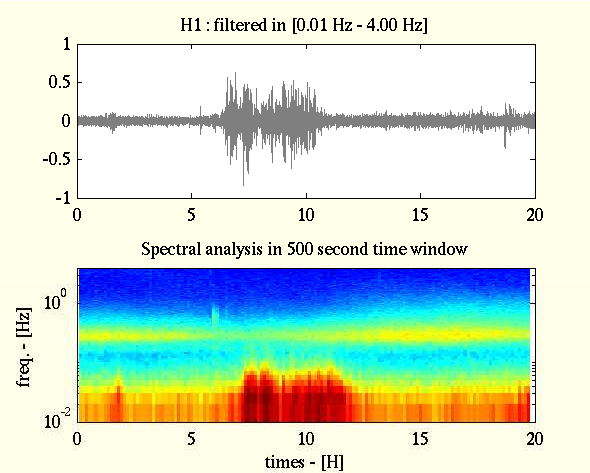
\includegraphics[scale=0.8]{../figures/tempspectanalysisH1LOWI3720140906.pdf}
&
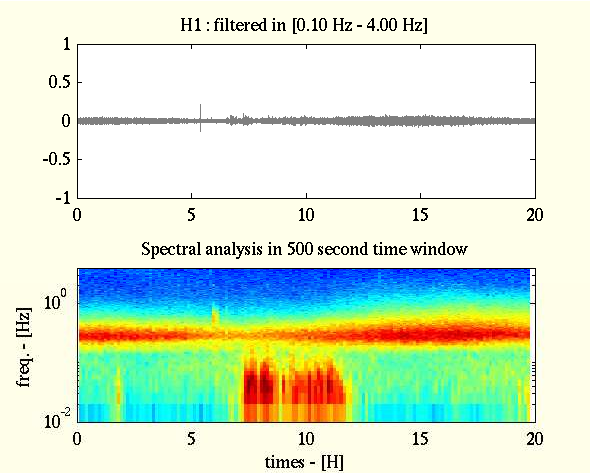
\includegraphics[scale=0.8]{../figures/tempspectanalysisH1HIGHI3720140906.pdf}
\end{tabular}
\begin{center}
\parbox{14 cm}
{
    \caption{\protect\small\it  {Typical observations on I37 during about $20$ hours. The signals are filtered in the band $0.01$ Hz to $4$ Hz and in the band $0.1$ Hz to $4$ Hz. The plot im grey represents the time observations. The color image represents the spectral analysis. The analysis time window is $500$ seconds. A low frequency components appears on the left figures. A common frequency component appears around the frequency band $[0.2-0.3]$ Hz}}
    \label {fig:tempspectanalysisI3720140905}
}
\end{center}
\end{table}

%Figure \ref{fig:tempspectanalysisI3720140905}, we observe an almost permanent component around $0.04$ Hz and another around $0.28$ Hz. We also observe bursts in red in the low frequency. These bursts present a low coherence between them as we see figure \ref{}.

\newpage

\newcommand{\paquet}[2]{
%==================================================================
\begin{table}[h]
\begin{center}
\begin{tabular}{c}
{\bf In the band $0.05$ Hz to $0.1$ Hz and in the band $0.25$ Hz to $0.3$ Hz}
\\
\includegraphics[scale=0.66]{../figures/#1}
\\
\includegraphics[scale=0.66]{../figures/#2}
\end{tabular}
\parbox{14cm}
{\it\small LHS figures: on top, the two nearest sensor signals. Bottom: time slots where the MSC is greater than $0.9$ for the different frequencies in the band $0.05$ Hz to $0.1$ Hz and in the band $0.25$ Hz to $0.3$ Hz. RHS figure: the decay of the MSC for the different frequencies reported on the LHS bottom figure as a function of the $10\times 9/2=45$ values of $f^2d^2$.  In the model given by \eqref{eq:logMSCgaussianmodel}, the intercept is related to the SNR.}
\end{center}
\end{table}}
%\subsubsection{In the band $0.05$ Hz to $0.1$ Hz/In the band $0.25$ Hz to $0.3$ Hz}

%==================================================================

\paquet{coherence2nearestI3720140902LOW.pdf}{coherence2nearestI3720140902HIGH.pdf}

%%==================================================================
\paquet{coherence2nearestI3720140903LOW.pdf}{coherence2nearestI3720140903HIGH.pdf}
%
%%==================================================================
\paquet{coherence2nearestI3720140904LOW.pdf}{coherence2nearestI3720140904HIGH.pdf}
%
%%==================================================================
\paquet{coherence2nearestI3720140905LOW.pdf}{coherence2nearestI3720140905HIGH.pdf}
%
%%==================================================================
\paquet{coherence2nearestI3720140906LOW.pdf}{coherence2nearestI3720140906HIGH.pdf}
%
%%==================================================================
\paquet{coherence2nearestI3720140907LOW.pdf}{coherence2nearestI3720140907HIGH.pdf}
%
%%==================================================================
\paquet{coherence2nearestI3720140908LOW.pdf}{coherence2nearestI3720140908HIGH.pdf}
%
%%==================================================================
\paquet{coherence2nearestI3720140909LOW.pdf}{coherence2nearestI3720140909HIGH.pdf}
%
%%==================================================================

 \newpage\clearpage
%=======================================================
 \section{Cramer-Rao bound (CRB)}
%=======================================================
%=======================================================
Let us consider a statistical model associated to an $N$ dimensional observation $X$, whose log-likelihood function writes $\ell(x;\alpha)$ where $\alpha$ is a $L$-dimensional parameter. Then any unbiased estimator $\hat\alpha_{N}$ of $\alpha$ has a covariance matrix which verifies:
\begin{eqnarray*}
 \esp{(\hat\alpha_{N}-\alpha) (\hat\alpha_{N}-\alpha)^{T}}&\leq& \mathrm{CRB}(\alpha) = F^{-1}(\alpha)
\end{eqnarray*}
where $F$ is called the Fisher information matrix (FIM) whose $(m,m')$ entry writes:
\begin{eqnarray*}
 F_{m,m'}&=&\esp{\nabla_{\alpha}\ell(x;\alpha)\nabla_{\alpha}^{T}\ell(x;\alpha)}
\end{eqnarray*}
where $\nabla_{\alpha}\ell(x;\alpha)$ is the gradient of $\ell(x;\alpha)$ w.r.t. $\alpha$. It is worth to notice that $F$ is $L$ dimensional square matrix.


 \bigskip
In the Gaussian case given by the expression \eqref{eq:likelihood-function}, it is shown:
\begin{eqnarray}
 \label{eq:FIMgaussian}
\fim_{m,m'}(\alpha)&=&\sum_{k=1}^{K}\trace{\Gamma_{k}^{-1}\times\partial_{m}\Gamma_{k}\times\Gamma_{k}^{-1}\times\partial_{m'}\Gamma_{k}}
\end{eqnarray}
where $1\leq m,m'\leq K+4$ and where $\partial_{\ell}\Gamma_{k}$ is the partial derivative w.r.t. $\alpha$.   We let:
\begin{eqnarray*}
 \dot d_{k,m}(\theta)&=&
  \begin{bmatrix}
  -2j\pi f_{k} r_{1,m}\,e^{-2j\pi f_{k}r_{1}^{T}\theta}
  \\
  \vdots
  \\
  -2j\pi f_{k} r_{M,m}\,e^{-2j\pi f_{k}r_{M}^{T}\theta}
  \end{bmatrix}
\end{eqnarray*}
Then for $m=1,2,3$:
\begin{eqnarray*}
\partial_{m}\Gamma_{k}&=&
   \gamma_{k}\diag{ \dot d_{k,m}(\theta)}C_{k}(\beta)D_{k}^{H}(\theta)+
   \gamma_{k} D_{k}(\theta)C_{k}(\beta) \diag{ \dot d_{k,\ell}(\theta)}^{H}
   \\
   &=&2\, \gamma_{k} \mathcal{R}\left(
   \diag{d_{k,m}(\theta)}C_{k}(\beta)D_{k}^{H}(\theta)\right)
\end{eqnarray*}
It is worth to notice that, if $\beta\approx +\infty$, $C_{k}=I_{M}$ and $\partial_{\ell}\Gamma_{k}=0$ which is normal because in this case $\Gamma_{k}$ does not depend on $\theta$. For the derivation w.r.t. $\sigma^{2}$ we have:
\begin{eqnarray*}
\partial_{4}\Gamma_{k}&=&I_{M}
\end{eqnarray*}
A direct consequence is that the FIM, w.r.t. the components \eqref{eq:alphareducted} of $\alpha$ is of this shape:
\begin{eqnarray*}
 \fim&=&\begin{bmatrix}
 F_{11}&F_{12}&F_{13}&0&0&\ldots&0
 \\
 F_{21}&F_{22}&F_{23}&0&0&\ldots&0
 \\
F_{31}&F_{32}&F_{33}&0&0&\ldots&0
 \\
0&\ldots&0&F_{\sigma^{2}}&
 \\
0&\ldots&0&&
\\
\vdots&\ddots&\vdots&&&F_{\gamma,K,K}
\\
0&\ldots&0
 \end{bmatrix}
\end{eqnarray*}
Because the CRB on the estimation of $\theta$ is given by the $3\times 3$ top-left matrix of the inverse of $\fim$, we are only concern with $ F_{123}$ by taking $ F_{123}^{-1}$ . Then the CRB w.r.t. the azimuth, elevation and velocity can be derived using the Jacobian of the one-to-one mapping between the slowness and the vector $(a,e,c)$ where $a$, $e$ and $c$ denote respectively the azimut, the elevation and the velocity. The same calculation can be used to derive the CRB w.r.t. the azimuth and the trace velocity.


%=======================================================
%=======================================================
\chapter{Appendix}
\section{Transform an array in isotrope array}
We consider an arbitrary  array whose locations are given by:
\begin{eqnarray*}
X&=&\begin{bmatrix}
x_{1,1}&\ldots&x_{1,M}
\\
x_{2,1}&\ldots&x_{2,M}
\\
x_{3,1}&\ldots&x_{3,M}
\end{bmatrix}
\end{eqnarray*}
It follows that
\begin{eqnarray*}
 XX^{T}&=&
 \sum_{i=1}^{d}\mu_{i}\xi_{i}\xi^{T}_{i}
\end{eqnarray*}
where $0\leq \mu_{i}\leq \alpha_{0}$. The new array writes
\begin{eqnarray*}
Y &=& \begin{bmatrix}
X&\sqrt{(\alpha_{0}-\mu_{1})}\xi_{1}&\sqrt{(\alpha_{0}-\mu_{2})}\xi_{2}&\sqrt{(\alpha_{0}-\mu_{3})}\xi_{3}
\end{bmatrix}
\end{eqnarray*}
It is easy to verify that $YY^{T}=\alpha_{0}I_{d}$.

It is worth to notice that this isotropy is related to the 3 components of the slowness vector. If we used another parametrization, as for example azimuth, elevation, velocity we have to reconsidered the solution taking into account the Jacobian of the transformation.

%=======================================================
%=======================================================
\section{Loss of coherence (LOC)}
The LOC is modeled by the randomness of the slowness vector as:
\begin{eqnarray*}
\Theta &=& \theta_0+\epsilon
\end{eqnarray*}
where $\theta_0$ is a 3D deterministic vector and $\epsilon$ a 3D random vector with zero-mean and distribution probability density denoted $p_{\epsilon}$. The spectral matrix entry of the $M$-ary random vectors associated to the sensor pair location $r_{m}$ and $r_{m'}$, writes:
\begin{eqnarray*}
S_{m,m'}(f) &=& \gamma(f)\int_{\mathds{R}^3}e^{-2j\pi f (r_{m}-r_{m'})^Tt}p_{e}(t-\theta_0)dt
\\
&=&\gamma(f)
e^{-2j\pi f (r_{m}-r_{m'})^T\theta_0}
\int_{\mathds{R}^3}e^{-2j\pi f (r_{m}-r_{m'})^Tt}p_{e}(t)dt
\\
&=&\gamma(f)
e^{-2j\pi f (r_{m}-r_{m'})^T\theta_0}\times
\Phi_{e}(2\pi f(r_{m}-r_{m'}))
\end{eqnarray*}
where $\Phi_{e}(v)$ denotes the characteristic function of the r.v. $e$. The expression of the matrix $S$ writes:
\begin{eqnarray}
\label{eq:spectralmatrixwithequaldensity}
 S(f) &=& \gamma_s(f)D(f)C(f)D^H(f)
\end{eqnarray}
$D(f)$ is a diagonal matrix whose the $m$-th diagonal entry is $e^{-2j\pi f r_{m}^T\theta_0}$ and $C(f)$ a matrix whose the $(m,m')$-entry writes:
\begin{eqnarray*}
 C_{m,m'}(f) &=& \Phi_{e}(2\pi f(r_{m}-r_{m'}))
\end{eqnarray*}

If the distribution of $\epsilon$ is symmetric, the matrix $C$ is real valued.


The expression \eqref{eq:spectralmatrixwithequaldensity} can be a little bit more generalized by taking into account different spectral distribution on the $M$ sensors:
\begin{eqnarray*}
 \Gamma_{x}(f)&=&D(f)\Gamma_{s}(f)C(f)\Gamma_{s}(f)D^{H}(f)+ \sigma^{2}I_M
\end{eqnarray*}
where $\Gamma_{s}(f)$ is a diagonal matrix whose the $m$-th diagonal entry is $\gamma_{m}^{1/2}(f)$ meaning that the SOI arrives on each sensor with different spectral content. In most cases when the SOI is very far away from the station, we can consider that $\gamma_{m}(f)$ does not depend on $m$.


%=======================================================
%=======================================================
\subsubsection{Deterministic case}
%=======================================================
The deterministic case meaning $\epsilon=0$ leads to:
\begin{eqnarray*}
S_{m,m'}(f) &=& \gamma(f)e^{-2j\pi f (r_{m}-r_{m'})^T\theta_0}
\end{eqnarray*}
and therefore $S(f)=d(f)d^H(f)$ where $d$ is a complex vector whose the $m$-entry writes $e^{-2j\pi f r_{m}^T\theta_0}$. Hence $S$ is a projector of rank 1 and corresponds to a pure coherent case.

%=======================================================
%=======================================================
\subsubsection{Gaussian case}
%=======================================================
If we assume that $\epsilon$ is gaussian with covariance matrix $S_{\theta}$:
\begin{eqnarray*}
 \Phi_{e}(2\pi f(r_{m}-r_{m'}))&=& e^{-2\pi^2f^2 (r_{m}-r_{m'})^TS_{\theta}(r_{m}-r_{m'})}
\end{eqnarray*}
$S_{\theta}$ depends on 6 free parameters. Using \eqref{eq:MSCgeneralmodel} and in the absence of noise, the log MSC writes:
\begin{eqnarray}
\label{eq:MSCgaussianwithoutnoise}
 \log \MSC(f) &=& -4\pi^2f^2 (r_{m}-r_{m'})^TS_{\theta}(r_{m}-r_{m'})
\end{eqnarray}

\begin{remark}[Unities]
the covariance matrix $S_{\theta}$ is in s$^2$/m$^2$. It follows that $f^2 S_{\theta}$ is homogeneous at the inverse of the wavelength square.
\end{remark}


%=======================================================
%=======================================================
\subsubsection{Estimation of the parameters of $S_{\theta}$}
%=======================================================
Considering the gaussian case for the slowness vector, and reporting the expression \eqref{eq:MSCgaussianmodelwithnoise}, we can write: 
\begin{eqnarray*}
 \log C_{k,m,m'} &=&
-2\log(1+\SNR_k^{-1})
-4\pi^{2} f_{k}^{2}(r_{m}-r_{m'})^{T}S_{\theta}(r_{m}-r_{m'})
 \\
 &=&
-2\log(1+\SNR_k^{-1})
-4\pi^{2} f_{k}^{2}(r_{m,1}-r_{m',1})^{2}S_{11}
-4\pi^{2} f_{k}^{2}(r_{m,2}-r_{m',2})^{2}S_{22}
\\&&
-8\pi^{2} f_{k}^{2}(r_{m,1}-r_{m',1})(r_{m,2}-r_{m',2})S_{12}
\\
&=&
\beta_{0}(k)
+\mu_{1}(k,m,m')S_{11}
+\mu_{2}(k,m,m')S_{22}
+2\mu_{3}(k,m,m')S_{12}
\end{eqnarray*}
which is linear w.r.t. the parameters $\beta_{0}(k)$, $S_{11}$, $S_{22}$ and $S_{12}$. That provides an easy way to estimate.
Enumerating the frequency index, $k=1:K$, the sensor index $m=1:M$, $m'=1:M$ with $m'>m$ leads to $KM(M-1)/2$ equations with $K+3$ unknowns.
If we assume that $S_{\theta}=sI_3$, and the SNR does not depend on $k$, the expression simplifies:
\begin{eqnarray*}
 \log C_{k,m,m'} &=&
-2\log(1+\SNR^{-1})
-4\pi^{2} f_{k}^{2}(r_{m,1}-r_{m',1})^{2}s
\\
&=&\beta_{0}+\beta_{1}f_{k}^{2}(r_{m,1}-r_{m',1})^{2}
\end{eqnarray*}
which is \eqref{eq:simplemodelMSC}.
%=======================================================
%=======================================================
\subsubsection{Expression in azimut, elevation, velocity}
Using \eqref{eq:jacobianaec2theta}, we can derive an expression for the LOC in terms of azimuth $a$, elevation $e$ and velocity $c$. We have:
\begin{eqnarray}
\label{eq:theta2aec}
S_{\theta}=J\,S_{\aec}\,J^{T}
\end{eqnarray}
Then
\begin{eqnarray*}
 \log \Phi_{e}(2\pi f(r_{m}-r_{m'}))&=& 
-2\pi^2\frac{f^2}{c^2} (r_{m}-r_{m'})^TK(a,e,c)S_{\aec}K^T(a,e,c)(r_{m}-r_{m'})
\\
&=&
-2\pi^2(\rho_{m}-\rho_{m'})^TK_{\aec}S_{\aec}K^T_{\aec}(\rho_{m}-\rho_{m'})
\end{eqnarray*}
where $\rho=r/\lambda$ with $\lambda=c/f$ and
\begin{eqnarray*}
K_{\aec}&=&
\begin{bmatrix}
\cos(a)\cos(e)&\sin(a)\sin(e)&c^{-1}\sin(a)\cos(e)
\\
-\sin(a)\cos(e)&-\cos(a)\sin(e)&-c^{-1}\cos(a)\cos(e)
\\
0&\cos(e)&-c^{-1}\sin(e)
\end{bmatrix}
\end{eqnarray*}
A simple case is if we take $S_{\aec}$ diagonal and hence depending on only 3 free parameters. 

%=======================================================
%=======================================================
\section{One-to-one mappings and Jacobians}
%=======================================================
\subsubsection{$\theta$ to $(a,e,c)$ }
If we consider the one-to-one mapping $\theta$ to $(a,e,c)$ in $(0,2\pi)\times(-\pi/2,\pi/2)\times\mathds{R}^+$, we can write:
\begin{eqnarray*}
\begin{array}{cc}
 \left\{
 %\renewcommand\arraystretch{1.2}
 \begin{array}{ll}
 \theta_{1}=-c^{-1} \sin(a)\cos(e)&\, \theta_{1}\in\mathds{R}
 \\
 \theta_{2}=c^{-1}  \cos(a)\cos(e)&\,\theta_{2}\in\mathds{R}
 \\
 \theta_{3}=c^{-1}\sin(e)&\, \theta_{3}\in\mathds{R}
 \end{array}\right.
&
 \left\{
 \begin{array}{ll}
 a=\arg(\theta_{2}-j \theta_{1})& \, a\in(0,2\pi)
  \\
e=\arg\sin(c\theta_{3})& \,e\in(-\pi/2,\pi/2)
 \\
 c=(\theta_{1}^{2}+ \theta_{2}^{2}+ \theta_{3}^{2})^{-1/2}& \, c \geq 0
 \end{array}\right.
\end{array}
\end{eqnarray*}
whose the Jacobian is
\begin{eqnarray}
 \label{eq:jacobianaec2theta}
 J(a,e,c)
&= &
 \begin{bmatrix}
-c^{-1}\cos(a)\cos(e)&c^{-1}\sin(a)\sin(e)&c^{-2}\sin(a)\cos(e)
\\
-c^{-1}\sin(a)\cos(e)&-c^{-1}\cos(a)\sin(e)&-c^{-2}\cos(a)\cos(e)
\\
0&c^{-1}\cos(e)&-c^{-2}\sin(e)
\end{bmatrix}
\\
&=&\nonumber
c^{-1}
\begin{bmatrix}
\cos(a)\cos(e)&\sin(a)\sin(e)&c^{-1}\sin(a)\cos(e)
\\
-\sin(a)\cos(e)&-\cos(a)\sin(e)&-c^{-1}\cos(a)\cos(e)
\\
0&\cos(e)&-c^{-1}\sin(e)
\end{bmatrix}
\\
&=&\nonumber
c^{-1}K_{\aec}
\end{eqnarray}

\subsubsection{$\theta$ to $(a,e,v)$ }
If we consider the one-to-one mapping $\theta$ to $(a,e,v)$ in $(0,2\pi)\times(-\pi/2,\pi/2)\times\mathds{R}^+$, we can write:
\begin{eqnarray*}
\begin{array}{cc}
 \left\{
 %\renewcommand\arraystretch{1.2}
 \begin{array}{ll}
 \theta_{1}=-v^{-1} \sin(a)&\, \theta_{1}\in\mathds{R}
 \\
 \theta_{2}=v^{-1}  \cos(a)&\,\theta_{2}\in\mathds{R}
 \\
 \theta_{3}=v^{-1}\tan(e)&\, \theta_{3}\in\mathds{R}
 \end{array}\right.
&
 \left\{
 \begin{array}{ll}
 a=\arg(\theta_{2}-j \theta_{1})& \, a\in(0,2\pi)
  \\
e=\arg\tan(v\theta_{3})& \,e\in(-\pi/2,\pi/2)
 \\
 v=(\theta_{1}^{2}+ \theta_{2}^{2})^{-1/2}& \, c \geq 0
 \end{array}\right.
\end{array}
\end{eqnarray*}
whose the Jacobian is
\begin{equation}
 \label{eq:jacobianaecv2theta}
 J(a,e,v)
 = 
 \begin{bmatrix}
-v^{-1}\cos(a)&0&v^{-2}\sin(a)
\\
-v^{-1}\sin(a)&0&-v^{-2}\cos(a)
\\
0&v^{-1}/\cos^2(e)&-v^{-2}\tan(e)
\end{bmatrix}
\end{equation}

%%=======================================================
%%=======================================================
%\chapter{inverse of $\Gamma_{k}$}
%%=======================================================
%Here we give the analytical expression of the inverse of $\Gamma_{k}(\alpha)=\gamma_{k}D_{k}(\theta)\, C_{k}\,D_{k}^{H}(\theta)+\sigma^{2}I_{M}$
%\begin{eqnarray*}
%\Gamma_{k}^{-1}(\alpha)&=&
%\sigma^{-2}I_{M}-\sigma^{-4}D_{k}(\theta)(C_{k}^{-1}+\sigma^{-2}D_{k}^{H}(\theta)D_{k}(\theta))^{-1}D_{k}^{H}(\theta)
%\\
%&=&
%\sigma^{-2}I_{M}-\sigma^{-4}D_{k}(\theta)(C_{k}^{-1}+\sigma^{-2}I)^{-1}D_{k}^{H}(\theta)
%\end{eqnarray*}

\end{document}

